\documentclass[a4paper]{scrartcl}
\usepackage[utf8]{inputenc} % use utf8 file encoding for TeX sources
\usepackage[T1]{fontenc}    % avoid garbled Unicode text in pdf
\usepackage[german]{babel}  % german hyphenation, quotes, etc
\usepackage{hyperref}       % detailed hyperlink/pdf configuration
\usepackage{amsfonts}
\usepackage{array} % for "\newcolumntype" macro
\usepackage{pgfplots}
\pgfplotsset{compat=1.8}
\usepackage{pst-plot}
\usepackage{pst-eucl}
\newcolumntype{L}{>{\centering\arraybackslash}m{2.8cm}}

\newcolumntype{M}{>{\centering\arraybackslash}m{5.7cm}}
\usepackage{amsmath}
\graphicspath{ {.} }

\pagestyle{headings}
\pagenumbering{gobble}

\hypersetup{                % ‘texdoc hyperref‘ for options
pdftitle={Analysis 1}
}
\usepackage{graphicx}       % provides comman ds for including figures
\usepackage{csquotes}       % provides \enquote{} macro for "quotes"
\usepackage[nonumberlist]{glossaries}     % provides glossary commands
\usepackage{enumitem}

\title{Analysis Formelsammlung}

\begin{document}
    \maketitle
    \newpage
    \tableofcontents
    \newpage
    
    \section{Komplexe Zahlen}
        \subsection{Definitionen}
            \subsubsection{Definitionen}
                Die Menge der Komplexen Zahlen werden mit dem Symbol \(\mathbb{C}\) beschrieben.\\
                Sei \(z\) ein Element aus \(\mathbb{C}\) so gilt:
                \begin{equation*}
                    z \, \epsilon \, \mathbb{C} : (z = x + iy \,|\, x,y \,\epsilon \, \mathbb{R})
                \end{equation*}
                Wobei \(x\) der reelle Anteil und \(y\) der imaginäre Anteil der komplexen Zahl ist. \\
                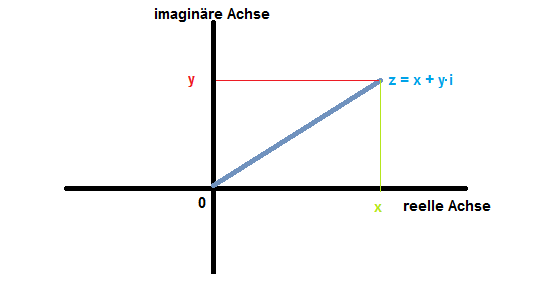
\includegraphics{c}
            
            \subsubsection{Formen}    
                \begin{description}
                    \item[Kartesische Form] $z = x + y*i$
                    \item[Trigonometrische Form]   $r(cos\varphi + i*sin\varphi)$
                    \begin{description}
                        \item[Herleitung:]  Es gilt: \(x = r * \cos\varphi, \, y = r * \sin\varphi \\
                        z = x + i*y = r * cos\varphi + i * r* sin\varphi = r(cos\varphi + i*sin\varphi) \), 
                        \\ $r = |z|$ 
                        \item[Berechnung von $\varphi$:] Je nachdem, in welchem Quadranten sich $z$ befindet, ändert sich die Formel leicht um $\varphi$ zu bestimmen.\\
                            Allgemein gilt $sin \varphi = \cfrac{y}{|z|} \rightarrow \varphi = arcsin(\cfrac{y}{|z|})$
                        \begin{itemize}
                            \item Quadrant 1: $\varphi = \varphi_{Rechenr}$
                            \item Quadrant 2 : $\varphi = \pi - \varphi_{Rechner}$
                            \item Quadrant 3 : $\varphi = \pi + |\varphi_{Rechner}|$
                            \item Quadrant 4: $\varphi = \varphi_{Rechner}$
                        \end{itemize}
                    \end{description}
                    \newpage
                    \item[Exponentialform] $r * e^{i\varphi}$ 
                    \begin{description}
                        \item[Herleitung:] Es gilt:\(e^{i\varphi} = cos\varphi + i * sin\varphi \) \\ \(z = r * (e^{i\varphi} = cos\varphi + i * sin\varphi) = r * e^{i\varphi} \), $\varphi$ wird wie oben berechnet.
                    \end{description}
                \end{description}          

            \subsubsection{Grundrechenarten}
                \begin{description}
                    \item[Addieren] $z_1 + z_2 = x_1 + x_2 + (y_1 + y_2)*i$ 
                    \item[Subtrahieren] $z_1 - z_2 = x_1 - x_2 + (y_1 - y_2)*i$ 
                    \item[Multiplizieren] beim Multiplizieren wird unterschieden ob mit einem konstanten Faktor oder einer weiteren komplexen Zahl multipliziert wird.
                    \begin{itemize}
                        \item mit einem Faktor a: $a * z = a * x + a * y * i $
                        \item mit einer Komplexen Zahl z_2: $z_1 * z_2 = x_1 * x_2 - y_1 * y_2 + (x_1 * y_2 + x_2 * y_1) * i $
                    \end{itemize}  
                    \item[Dividieren]  $\cfrac{z_1}{z_2} = \cfrac{x_1*x_2 + y_1*y_2 + (-x_1*y_2 + x_2*y_1)*i}{x_2^{\;\;2} + y_2^{\;\;2}}$
                    \item[Betrag] $|z| = (x^2 + y^2)^\frac{1}{2} = \sqrt{x^2 + y^2}$ 
                    \item[Komplex Konjugiert] $z = x \pm y*i \rightarrow z^* = x \mp y*i$ 
                \end{description}
                
            \subsubsection{Radizieren}
            Wenn aus einer Komplexen Zahl z die n-te Wurzel gezogen wird, entstehen somit auch n verschiedene Wurzeln.
            Die allgemeine Formel dafür lautet 
            \begin{equation*}
                z^{\frac{1}{n}} = |z|^{\frac{1}{n}} * e^{i(\frac{\varphi}{n} + \frac{m}{n}* 2\pi)}
            \end{equation*}
            Das $n$ bleibt immer konstant und $m$ startet bei 0 und wird bis $m = n-1$ hochgezählt, wodurch man die $n$ Wurzel herbekommt,
            lediglich $\varphi$ und $|z|$ müssen wie oben beschrieben berechnet werden und ggf. muss $z$ in die Exponentialform gebracht werden, um die Berechnungen zu erleichtern.  
        \newpage
    \section{Funktionen}

    \subsection{Nullstellen}
    $f(x)$ hat Nullstellen wenn gilt $x_0$  $f(x_0) = 0$

    \subsection{Symmetrie}
    \begin{description}
        \item Eine Funktion heißt gerade (spiegelsymmetrisch) wenn gilt: $f(-x) = f(x)$ 
        \item Eine Funktion heißt ungerade(punktsymmetrisch): $f(-x) = -f(x)$
    \end{description}
    
    \subsection{Monotonoie} 
    Die Definition für die Monotonie wird unten aufgelistet. Es gilt außerdem: $x_1 < x_2 $ 
    \begin{itemize}
        \item monoton wachsend:  $f(x_1) \leq f(x_2)$
        \item streng monoton wachsend: $f(x_1) < f(x_2)$
        \item monoton fallend:  $f(x_1) \geq f(x_2)$
        \item streng monoton fallend:  $f(x_1) > f(x_2)$
    \end{itemize}
    
    \subsection{Periodizät}
    Wenn ein $p$ existiert für das gilt $f(x \pm p) = f(x)$ und $x \pm p$ ist im Definitionsbereich, ist $f$ periodisch mit der Periode $p$,\\
    $p$ kann auch $\pm k \, * \,p$ sein, wobei $k \, \epsilon \, \mathbb{N}^*$. Kleinstes positives $p$ nennt man die primitive Periode
    
    \subsection{Umkehrfunktion}
    Funktion f heißt umkehrbar wenn gilt:     
    \begin{description}
        \item $x_1 \neq x_2 \rightarrow f(x_1) \neq f(x_2)$ oder
        \item wenn f streng monoton ist.
        \end{description}
    Definitions- und Wertebereich sind bei der Umkehrfunktion "vertauscht". \\  
    \\ Um die Umkehrfunktion zu bestimmen, formt man $f(x)$ nach $x$ um und vertauscht danach $x$ und $y$ wodurch man $f^{-1}$ erhält.
    Oft muss der Definitionsbereich dabei eingeschränkt werden, da z.B. die Parabel nur für $x \geq 0$ monoton ist (bzw. $x \leq 0$). 

    \subsection{Grenzwert einer Funktion}
    Existiert ein $g$ für das gilt:
    \begin{equation*}
        \lim \limits_{n \to \infty}f(x_n) = g
    \end{equation*} 
    so ist $g$ der Grenzwert von $f$.
    $x_n$ wird durch den limes immer höher, $g$ kann auch gegen unendlich gehen und $g$ muss auch nicht im Wertebereich liegen. Wenn $g$ nicht im Wertebereich liegt, so ist $g$ auch die Asymptote. \\
    $\lim$ kann auch gegen $-\infty$ oder auch gegen einen Punkt gehen.

    \subsection{Stetigkeit einer Funktion}
        Eine Funktion heißt stetig im Punkt $x_0$:
        \begin{description}
            \item $f(x_0)$ ist definiert: Beispielsweiße ist $\cfrac{1}{x}$ nicht stetig in $\mathbb{R}$ jedoch in $\mathbb{R} \setminus 0$ da hier $x_0 = 0$ nicht definiert ist (nicht definierte Werte werden bei der Überprüfung der Stetigkeit nicht berücksichtigt)
            \item $lim_{x \to x_0}: f(x) existiert$: An allen definierten Punkten muss ein Grenzwert nach $x_0$ vorliegen. Es dürfen sozusagen keine Lücken vorhanden sein ($\cfrac{1}{x}$ mit $\mathbb{R}$ hat z.B. eine "Lücke" für $x_0 = 0$).
            \item $lim_{x \to x_0}: f(x) = f(x_0)$: Der Grenzwert an Stelle $x_0$ muss gleich dem Funktionswert an Stelle $x_0$ sein.
        \end{description}
        Ist eine Funktion in jedem Punkt stetig, heißt die komplette Funktion stetig.


    \subsection{Tabelle mit Funktionen und deren Eigenschaften}
        \subsubsection{Polynomfunktion}        
        \begin{description}
            \item[Definition] $f(x) = a_n*x^n...a_1*x + a_0$ wobei $n$ auch der Grad der Funktion ist
            \item[Symmetrie] Eine Polynomfunktion ist gerade, wenn alle Polynome eine gerade Potenz haben und ist ungerade, wenn alle Polynome ungerade Exponenten haben.
        \end{description}

        \subsubsection{Gebrochenrationale Funktion}
        \begin{description}
            \item[Funktion] $f(x) = \cfrac{g(x)}{h(x)}= \cfrac{a_m*x^m...a_1*x + a_0}{b_n*x^n...b_1*x + b_0}$ $g(x)$ unf $h(x)$ sind wiederum Polynomfunktionen. Außerdem wird unterschieden zwischen:
            \begin{itemize}
                \item $n > m$: echt gebrochenrational und
                \item $n \leq m$ unecht gebrochenrational
            \end{itemize}   
            \item[Nullstellen] $f(x)$ hat Nullstellen wo $g(x)$ Nullstellen hat aber $h(x) \neq 0$ ist.  
            \item[Pol] $f(x)$ hat Pole wo $h(x)$ Nullstellen hat. Wichtig ist, dass zuerst umgerechnet werden muss, da sich teilweise Terme aus dem Bruch rauskürzen können.
            Die Anzahl der Nullstellen in $h(x)$ wird mit $k$ bezeichnet und man spricht von eimem Pol $k$-ter Ordnung. Ist $k$
            gerade, gibt es keinen Vorzeichenwechsel am Pol, ist k ungerade gibt es einen Vorzeichenwechsel.
             \item[Asymptote] Um die Asymptote zu finden muss zuerst zwischen einer echten und unechten gebrochenrationalen Funktion unterschieden werden.
                \begin{itemize}
                    \item Echt gebrochenrational: hat eine Asymptote bei $y$ = 0.
                    \item Unecht gebrochenrational: $f(x)$ wird durch Polynomdivison in seine Linearkombination aufgeteilt. $f(x)$ kann nun in eine Polynomfunktion $p(x)$ und
                    eine echt gebrochenrationale Funktion $r(x)$ augeteilt werden  
                    \begin{equation*}
                        f(x) = p(x) + r(x)
                    \end{equation*}
                    $r(x)$ strebt gegen 0 weshalb die Asymptote von $p(x)$ gleich der Asymptote von $f(x)$ ist.
                \end{itemize}
             \item[Symmetrie] je nachdem welche Symmetrie die Polynomfunktionen haben ist auch die Symmetrie der gebrochenrationale Funktion anders. 
                \begin{itemize}
                    \item Haben $g(x)$ und $h(x)$ die gleiche Symmetrie ist $f(x)$ auch gerade.
                    \item Haben $g(x)$ und $h(x)$ verschiedene Symmetrien so ist $f(x)$ ungerade.
                    \item Haben entweder $g(x)$ oder $h(x)$ (oder beide) keine Symmetrie so hat $f(x)$ auch keine Symmetrie.
                \end{itemize}  
        \end{description}
        
        \subsubsection{Potenzfunktion}
           \begin{description}
               \item[Funktion] $f(x) = x^n$ 
               \item[Symmetrie] ist n gerade dann ist auch $f(x)$ gerade
               \begin{itemize}
                   \item Ist n gerade dann ist auch $f(x)$ gerade
                   \item Ist n ungerade dann ist auch $f(x)$ ungerade
               \end{itemize} 
           \end{description}       
    

           \subsection{Kurvendiskussion}
                \begin{description}
                    \item[Extrema] \(f'(x) = 0 \wedge f''(x) \neq 0\)
                    \begin{description}
                        \item[Maximum] \(f''(x) < 0\)
                        \item[Minimum]  \(f''(x) > 0\)
                    \end{description}
                    \item[Wendepunkt] \( f'(x) \neq 0 \wedge f''(x) = 0 \)
                    \item[Sattelpunkt] \(f'(x) = f''(x) = 0\) 
                \end{description}



    \section{Differentialrechnung}
        \subsection{Ableitungsregeln Funktion}
            \setlength{\arrayrulewidth}{0.5mm}
            \setlength{\tabcolsep}{16pt}
            \renewcommand{\arraystretch}{1.5}
            $\begin{array}{|l|c|c|}    
                    \hline
                    \textbf{Art der Funktion} & \textbf{Funktion} & \textbf{Ableitung}  \\
                    \hline
                    \hline
                    \text{Konstante Funktion}
                        & f(x) = c & f'(x) = 0 \\
                        \hline
                    \text{Gerade}              
                        & f(x) = x & f'(x) = 1 \\
                        \hline
                    \text{Potenzfunktion}      
                        & f(x) = x^n & f'(x) = n*x^{n-1} \\
                        \hline
                    \text{Exponentialfunktion}
                        & f(x) = a^x & f'(x) = ln(a) \cdot e^{ln(a)\cdot x} \\
                        & = e^{xln(a)} & f'(x) = ln(a) \cdot a^{x} \\
                        & f(x) = x^x = e^{x*ln(x)} & f'(x) = x^{x} * (ln(x)+1) \\
                        \hline
                    \text{Logarithmusfunktion} 
                        & f(x) = ln(x) & f'(x) = \cfrac{1}{x} \\
                        & f(x) = log_a(x) & f'(x) = \cfrac{1}{ln(a)*x} \\
                        \hline
                    \text{Trigonometrische Funktionen} 
                        & f(x) = sin(x) & f'(x) = cos(x) \\
                        & f(x) = cos(x) & f'(x) = -sin(x) \\
                        & f(x) = tan(x) & f'(x) = \cfrac{1}{cos^2(x)} = 1 + tan^2(x) \\
                        & f(x) = cotan(x) & f'(x) = -\cfrac{1}{sin^2(x)} = -1 - cotan^2(x) \\
                        \hline
                
                    \text{Arkusfunktionen} 
                        & f(x) = arcsin(x) & f'(x) = \cfrac{1}{\sqrt{1-x^2}} \\
                        & f(x) = arccos(x) & f'(x) = -\cfrac{1}{\sqrt{1-x^2}} \\
                        & f(x) = arctan(x) & f'(x) = \cfrac{1}{1+x^2} \\
                        & f(x) = arccotan(x) & f'(x) = -\cfrac{1}{1+x^2} \\
                        \hline
                \text{Hyperbelfunktion}    
                        & f(x) = sinh(x) & f'(x) = cosh(x) \\
                        & f(x) = cosh(x) & f'(x) = sinh(x) \\
                        & f(x) = tanh(x) & f'(x) = \cfrac{1}{cosh^2(x)} = 1-tanh^2(x) \\
                        & f(x) = coth(x) & f'(x) = -\cfrac{1}{sinh^2(x)} = 1 - coth^2(x) \\
                        \hline
                \text{Areafunktion} 
                        & f(x) = arsinh(x) & f'(x) = \cfrac{1}{\sqrt{1+x^2}} \\
                        & f(x) = arcosh(x) & f'(x) = \cfrac{1}{\sqrt{x^2-1}} \\
                        & f(x) = artanh(x) & f'(x) = \cfrac{1}{1-x^2} \\
                        & f(x) = arcotan(x) & f'(x) = \cfrac{1}{1-x^2} \\
                        \hline
            \end{array}$
            \newpage  
        \subsection{Ableitungsregeln Arithmetik}
                \begin{tabular}{|c|c|M|}
                    \hline
                    \textbf{Regeln}  & \textbf{Funktion} & \textbf{Ableitung}  \\
                    \hline
                    \hline
                    \text{Summenregel }
                        & f(x) = u(x) + v(x) & f'(x) = u'(x) + v'(x) \\
                    \hline
                    \text{Faktorregel}              
                        & f(x) = c * u(x) & f'(x) = c * u'(x) \\
                    \hline
                    \text{Produktregel}      
                        & f(x) = u(x) * v(x) & f'(x) = u'(x) * v(x) + u(x) * v'(x) \\
                    \hline
                    \text{Quotientenregel}
                        &  $f(x) = \cfrac{u(x)}{v(x)}$ & $f(x) = \cfrac{ u'(x) * v(x) - u(x) * v'(x)}{v(x)^2}$   \\
                    \hline
                    \text{Kettenregel} 
                        & f(x) = u(v(x)) & f = u'(v(x)) * v'(x) \\
                    \hline
                \end{tabular}
                
    \section{Integralrechnung}
        Die Integralrechnung ist die Umkehrung zur Differentialrechnung, weshalb man die Tabelle von der Differentialrechnung nutzen kann indem man sie von rechts nach links liest.
        Wird eine Funktion $f$ integriert erhält man die Stammfunktion $F$. Man schreibt auch:
        \begin{description}
            \item[Unbestimmtes Integral] $\int f(x) dx = F(x)$
            \item[Bestimmtes Integral] $\int_{a}^{b} f(x) dx = F(b) - F(a)$  wobei $a$ und $b$ das Intervall angeben in dem man integrieren möchte. 
        \end{description}
        \subsection{Rechenregeln}
            \begin{description}
                \item[Faktorregel] $\int c * f(x) dx = c * \int f(x) dx$ 
                \item[Summenregel] $\int f(x) + g(x) dx = F(x) + G(x)$  
            \end{description}
        \newpage
        \subsection{Integrationsmethoden}
        \begin{description}
            \item[Partielle Integration] $\int f(x) * g(x) dx = F(x) * g(x) - \int F(x) * g'(x) dx$ \\
             Hier sollte man schauen, dass man (wenn möglich) die Funktionen zum integrieren und differenzieren so wählt, dass sie im nächsten Schritt 'einfacher' werden.  
             Teilweise hilft es auch wenn nur $f(x)$ vorhanden ist, $g(x) = 1$ zu setzen da ja $1 * f(x) = f(x)$ ergibt.
             \item[Integration durch Substitution] $\int f(x)\, * \,g(x)\, dx = \,\int d(F(x) \,+ \,C) \,* \,g(x) \,dx$ 
             \\Sei nun $F(x) + C = u$  und $F(x) + C$ so gewählt dass man $u = g(x)$, 
            bzw. $u$ möglichst ähnlich zu $g(x)$ ist. Dann gilt wiedereum: $\int 1 * u \,du $ 
            \\Hier wurde jetzt $F(x)$ substituiert. Jetzt kann man, je nach Form der Gleichung schauen welche Regeln man anwenden kann, bzw. ob man in der Ableitungstabelle nachschauen ob direkt integriert werden kann.
            In diesem Fall kann man einfach integrieren: \\$\cfrac{1}{2}u^2$ jetzt wird noch rücksubstituiert und man kommt auf das Ergebnis: $\cfrac{1}{2}(F(x) + c)^2$
        \end{description}
\end{document}
